\section{The numbers}\label{sec:crit-calib}

The code is clean and reproduces everything, so each of the checks below took minutes. What they show is that the calibration is weaker than the text suggests, and that the numbers the abstract leads with are not the ones the calibration pins down.

\subsection{The reported parameters are not the best fit}

The parameter search runs on a coarse grid and re-ranks its candidates on a fine one. At the reported parameters the two grids disagree (a loss of 17.5 against 20.6). Started from another point, the same model reaches a loss of 13.8 on the paper's own fine grid.

\begin{center}\small
\begin{tabularx}{0.92\textwidth}{@{}Lrr@{}}
\toprule
 & Reported & Better optimum \\
\midrule
Loss on the fine grid & 20.6 & 13.8 \\
Speed limit $b_c$; mature density as a share of it & 38.6; 17\% & 43.2; 16\% \\
Planner's gain & 1.25\% & 1.06\% \\
Slope of the newcomer's payoff & 0.065 & 0.059 \\
Reading pass-through, no founders / founders & 14\% / 74\% & 13\% / 75\% \\
Newborn margin & 1.28\% & 0.10\% \\
Share of newborn topics that attract no follower & 36\% & 48\% \\
\bottomrule
\end{tabularx}
\end{center}

This sorts the paper's numbers by what survives. The incidence numbers, the small planner's gain and the distance from the speed limit survive. The newborn margin and everything built on it do not. The paper's sentence that exact catch-up ``makes the problem harder'' to fit is not supported: all of the apparent worsening relative to the previous version (14.9 to 20.6) is an unfinished search.

\subsection{The model does not reproduce the hump that motivates it}

\begin{figure}[h]
\centering
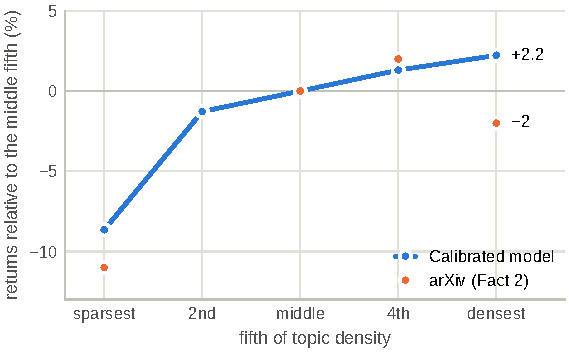
\includegraphics[width=0.66\textwidth]{fit.pdf}
\caption{Returns by fifth of topic density, relative to the middle fifth. In the data the densest fifth earns less than the middle. In the calibrated model returns rise all the way. (The paper does not report the second fifth for the data.)}
\label{fig:fit}
\end{figure}

A single-peaked payoff curve is the paper's founding object, and the hump in returns (Fact~2) is its motivation. In the calibrated model the observable cross-section has no falling arm.

\begin{itemize}
\item Returns are monotone across fifths of density in every parameter vector found. The densest fifth is between $+0.9\%$ and $+2.5\%$ against $-2\%$ in the data. It stays positive when that one moment is given 400 times its weight, and when concurrent overlap is added as a tenth parameter.
\item The paper's fit table compares unlike objects. For the data it reports the peak of a fitted quadratic (one standard deviation above the mean, with 12\% of researcher-years beyond). For the model it reports the peak of the latent payoff curve. Run the same regression on the model's data and the peak is at $+2.67$ standard deviations with 0.001\% of researcher-years beyond it.
\item The reason is structural. Dense topics in the model are the fertile ones, and a mature topic pays its insiders $F/\Gamma(\Pm)$, which \emph{rises} with density (Proposition~5). The cross-section traces the entry condition, not the payoff curve. The remedies the paper suggests (more erosion, concurrent overlap) cannot help.
\item Most of the little curvature the model does show comes from an assumed amount of measurement error in density (a log standard deviation of 0.3) that is hard-coded and not listed as a parameter. Without it the model's cross-section is essentially linear.
\end{itemize}

\begin{ideabox}[What would produce a falling arm]
The cross-topic variation in density would have to come from something that moves the newcomer's payoff but not the insider's: differences across topics in how costly it is to get in. Topics that are easy to enter would then be dense with their rents competed away, and the cross-section would trace the payoff curve itself. This is untested, but it is the natural use of the catch-up block.
\end{ideabox}

\subsection{Identification}

\begin{itemize}
\item \textbf{Nine parameters, eight targets.} One target (an incumbents' premium of 0.15) is assumed, not measured, and is unattainable at the calibrated curve, where the premium cannot exceed 0.119. Five of the eight come from one regression.
\item \textbf{What pins the speed limit.} Not the premium, as the paper's table says, but the share of researcher-years ``beyond the peak'', which is defined differently in the model and in the data, together with the assumed flow of newborn topics.
\item \textbf{What is loose.} The dispersion of diffusion rates is not identified at all. The median diffusion rate, the erosion parameter and the dispersion of fertility are weakly identified. The shares of researcher-years in growing and consolidating topics, and the share that overshoots, inherit this.
\item \textbf{No standard errors.} The loss is not a chi-square statistic. Its scales are tolerances (0.008 for the gradient, against a standard error of 0.0015 in the data).
\end{itemize}

\subsection{The reading share}

The target is 144 hours of article reading a year out of about 2,000, from a survey of all faculty. The model moment counts producing incumbents only (7.8\%). But the model also requires newcomers to read full time while they catch up, and that reading alone is 8.7\% of topic members' time, more than the whole 7\% budget. In total reading is 15.8\% of members' time and 13.2\% of all researcher-years. Either incumbents' reading share should be close to zero, or the catch-up block (a premium of 10\%, nine months of reading) is twice too large for the time-use data.

\subsection{Robust, fragile, artefact}

\begin{center}\small
\begin{tabularx}{\textwidth}{@{}P{1.12in}L@{}}
\toprule
\tsolid & \textbf{Hold across every fit, grid and assumption tried.}
The value of a tool at fixed topics (26.2 and 1.96 log points for 30\% tools; equal per hour).
Production above reading above catch-up, given the frontier assumption.
The planner's gain is small (0.15--1.25\%).
A stock-proportional tax beats a flat subsidy.
The economy is far from the speed limit. \\[4pt]
\tfragile & \textbf{Move with an unmeasured input or across equally good fits.}
14\%/74\% and 1.3--7.2 (0--93\% and 1.1--32 over the plausible range).
The catch-up pass-through (36--69\% across fits; 11--17\% on the life cycle).
The slope of the newcomer's payoff (0.021--0.123), and with it everything that divides by it.
The life-cycle shares (24\% growing, 20\% consolidating, 10\% beyond the peak). \\[4pt]
\tfails & \textbf{Artefacts of an arbitrary choice.}
The newborn margin (1.28\%), the 11\% bound on learning from the stock, ``a flat subsidy about equal to the margin'': the assumed birth flow.
The take-off threshold as a quantitative phenomenon: no topic is below it.
About two members per topic: the normalisation of $a$.
``Peak of $v$ at 0.70 against 1.00 in the data'': different objects.
``Mature topics at 17\% of the limit'': an identity in assumed rates. \\
\bottomrule
\end{tabularx}
\end{center}

\subsection{The stakes}

\begin{critbox}[What the paper can and cannot be about]
Every equilibrium effect in the calibrated model is about 1\% or less: the planner's gain (0.15--1.25\%), the best policy (0.72\%), stepping on toes (0.98--1.00). For reading tools the whole incidence question is whether 0.3 or 1.5 of 2.0 log points survive: a question about 1.2 log points per 30\% tool.

The large numbers are something else. 26.2 against 1.96 is the split of working time, 93\% to 7\%. The reversal under readership units is the same arithmetic in other units. The 11.2\% ``dissipated'' in the frictionless benchmark is a counterfactual the paper itself disowns. The 10\% insiders' premium is distribution, not efficiency.

So this is not a paper about a large distortion. On its own numbers ``innovation too fast'' costs about 1\% of output. It can be a paper about \emph{who gains}, about \emph{where growth lands}, and about two findings stated as such: the static misallocation is small, and crowding explains little of stepping on toes.
\end{critbox}
